\documentclass[addpoints,12pt,twoside]{exam} %answers 
\usepackage[paper=a4paper,left=15mm,right=15mm,top=25mm,bottom=25mm]{geometry}
\usepackage{graphicx}
%\usepackage[dvips]{graphicx}
\usepackage{floatflt,epsfig} 
\usepackage{ngerman}
\usepackage{german}
\usepackage[utf8]{inputenc}
\usepackage{amssymb, amsmath}
\usepackage[gate,ic,optics]{circ}
\usepackage{hyperref}

\usepackage{tikz,pgfplots}

\usepackage{graphicx}
%\usepackage{geometry}
\usepackage{calc}


\usepackage{qrcode} 
\usepackage{wrapfig}
\usepackage{gensymb}
\usepackage{siunitx}

\usepackage{color}
\definecolor{GridColor}{gray}{0.8}
\definecolor{SolutionBoxColor}{gray}{0.8}
\definecolor{SolutionColor}{rgb}{0.8,0.9,1}

\colorgrids
\colorsolutionboxes

%%MACROS 
\newcommand{\tdate}{23. April 2021}
\newcommand{\myqr}{\qrcode[hyperlink, height = 1cm]{https://github.com/shahrrks/myTutorium_tex/tree/main/Blatt_2}}
\newcommand\gauss[2]{1/(#2*sqrt(2*pi))*exp(-((x-#1)^2)/(2*#2^2))} % Gauss function, parameters mu and sigma
%%
\newcommand{\zt}{\textit{z(t)}}

\sisetup{
    locale = DE ,
    per-mode = symbol
}

\pagestyle{headandfoot}

\headrule
\footrule
\firstpageheader{ETIT-4}{\bfseries\Large {Übungsblatt 1}}{\tdate}
\runningheader{ETIT-4}
{Übungsblatt - 1}
{\tdate}
\firstpagefooter{ETIT-4}{Seite \thepage\ von \numpages}{\myqr}
\runningfooter{ETIT-4}{Seite \thepage\ von \numpages}{Shah Rrks}

\boxedpoints
%\pointpoints{Punkt}{Punkte}
\pointsinmargin
\marginpointname{\%}

\begin{document}
    %\setcounter{section}{1} %current page -1
    \author{Shah Rrks}
    \section*{Sys 1}
    \begin{questions}
        \question[12]
        In Abb.1 ist der zeitliche Verlauf des Signals \textit{z(t)} dargestellt. \textbf{alt Klausur}
    
            \begin{figure}[h]
            \centering
            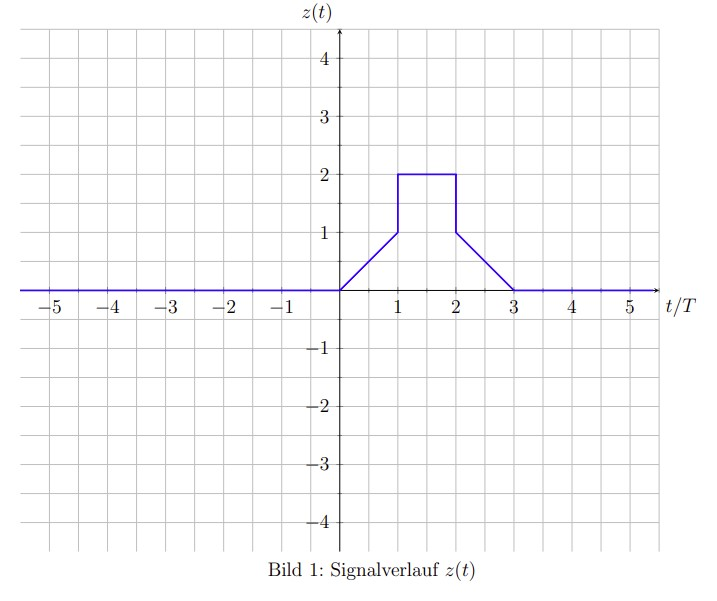
\includegraphics[width=0.8\textwidth]{auf1_signal}
            \caption{Signalverlauf z(t)}
            \label{fig:Signalverlauf-z-t-}
            \end{figure}
            \begin{parts}
                \part Bestimmen Sie die abschnittweise Definition von \textit{z(t)}
                \makeemptybox{2in}
                \part Berechnen Sie die Energie des Signals \zt. Handelt es sich hierbei um ein Energie- oder Leistungsignal ? 
                \begin{figure}[h]
                \centering
                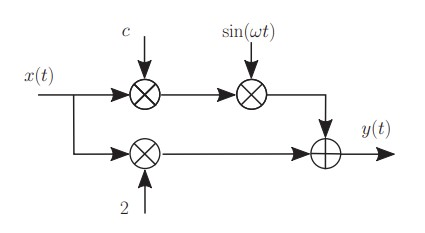
\includegraphics[width=0.4\textwidth]{blk}
                \caption{Blockdiagram}
                \label{fig:Blockdiagram}
                \end{figure}
                \part Bestimmen Sie für das in Bild 2 dargestellte System S das Ausgangssignal 
            \textit{y(t)}   in Abhängigkeit des Eingangssignal \textit{x(t)}. 
            \end{parts}
            
            \question[4]
            Summe Berechnen 
            \[ \sum_{n=1}^{\infty} \left( \frac{1}{3}  \right)^n
            \]
            \begin{figure}[h]
            %\centering
            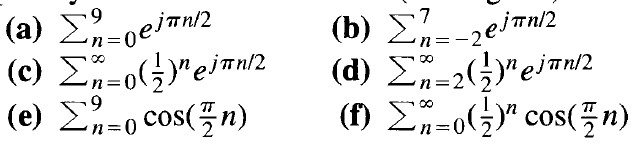
\includegraphics[width=0.5\textwidth]{auf2}
            \caption{ Summe Berechnen}
            \label{fig: Summe Berechnen}
            \end{figure}
            
            \question[6]
            Integrale Berechnen
            \begin{figure}[h]
            %\centering
            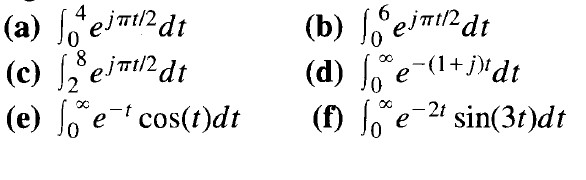
\includegraphics[width=0.5\textwidth]{auf3}
            \caption{Integrale Berechnen}
            \label{fig:Integrale Berechnen}
            \end{figure}

            
    \end{questions}
\newpage
    \section*{Info2}
	Boolsche Algebra Übungen (quelle:\url{ocw.mit.edu})
	\begin{figure}[h]
		\centering
		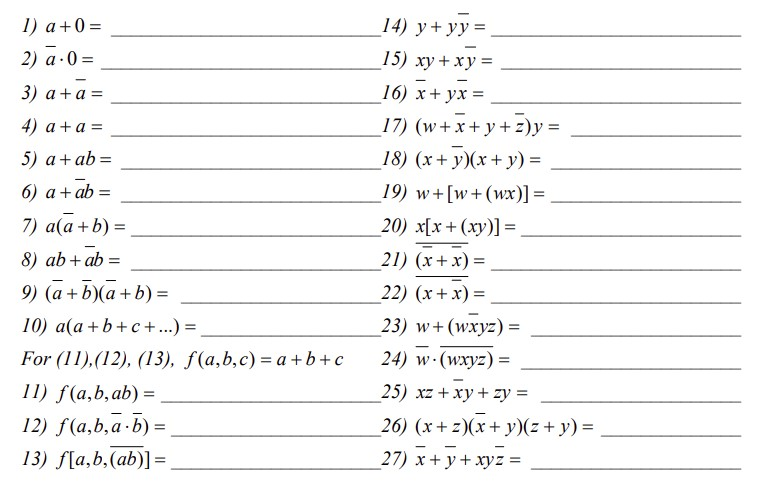
\includegraphics[width=1\linewidth]{bool_algebra}
	%	\caption{}
	\label{fig:boolalgebra}
	\end{figure}
\qrcode[hyperlink,height = 1.5cm]{https://github.com/shahrrks/myTutorium_tex/tree/main/Blatt_1_/FormelnZetteln} \hspace{5cm}
\qrcode[height = 1.5cm]{http://web.mit.edu/6.111/www/s2007/PSETS/pset1s.pdf}

\begin{figure}[h]
    \centering
    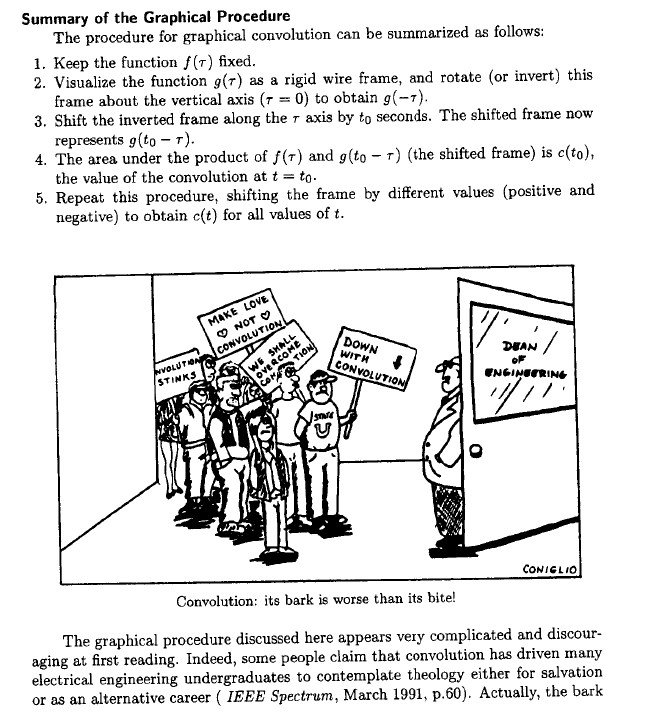
\includegraphics[width=1\textwidth]{conv}
    \caption{}
    \label{fig:}
    \end{figure}
\end{document}